\documentclass[border=12pt]{standalone}
\usepackage{tikz}
\usepackage{amsmath}
\usepackage{helvet}\renewcommand{\familydefault}{\sfdefault}
\usetikzlibrary{arrows.meta,positioning}
\begin{document}
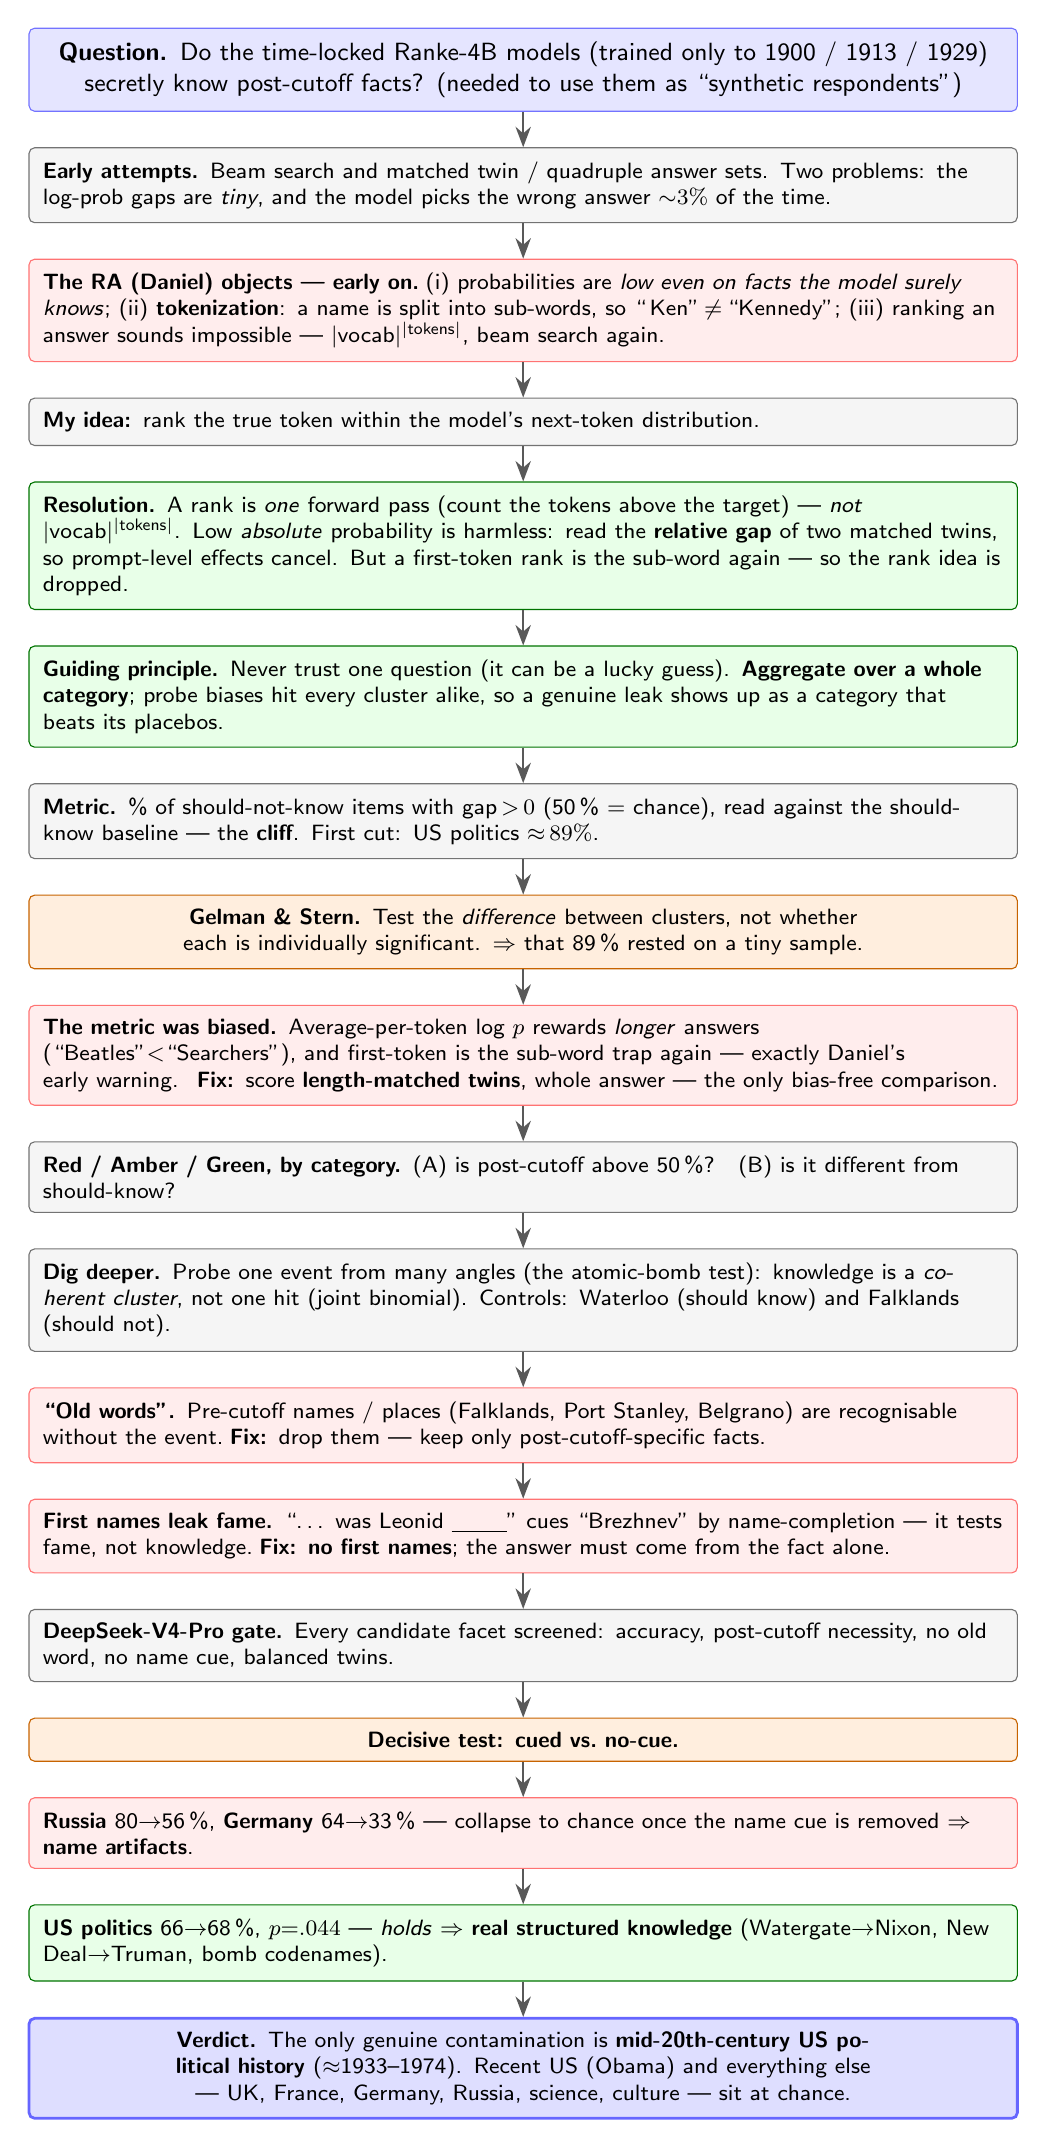
\begin{tikzpicture}[font=\footnotesize,
  box/.style={rectangle,rounded corners=2pt,draw=black!55,fill=black!4,text width=122mm,align=left,inner sep=5pt},
  start/.style={box,draw=blue!55,fill=blue!10,align=center,font=\small},
  verdict/.style={box,draw=blue!60,fill=blue!13,line width=1pt,align=center},
  find/.style={box,draw=red!55,fill=red!7},
  fix/.style={box,draw=green!45!black,fill=green!9},
  dec/.style={box,draw=orange!78!black,fill=orange!13,align=center},
  fl/.style={-{Stealth[length=2.6mm]},draw=black!65,line width=0.8pt},
  node distance=4.5mm,
]
\node[start](n1){\textbf{Question.} Do the time-locked Ranke-4B models (trained only to 1900 / 1913 / 1929) secretly know post-cutoff facts? (needed to use them as ``synthetic respondents'')};
\node[box,below=of n1](n2){\textbf{Early attempts.} Beam search and matched twin / quadruple answer sets. Two problems: the log-prob gaps are \emph{tiny}, and the model picks the wrong answer ${\sim}3\%$ of the time.};
\node[find,below=of n2](n3){\textbf{The RA (Daniel) objects --- early on.}\;(i)~probabilities are \emph{low even on facts the model surely knows}; (ii)~\textbf{tokenization}: a name is split into sub-words, so ``\,Ken''${\,\neq\,}$``Kennedy''; (iii)~ranking an answer sounds impossible --- $|\text{vocab}|^{|\text{tokens}|}$, beam search again.};
\node[box,below=of n3](n4){\textbf{My idea:} rank the true token within the model's next-token distribution.};
\node[fix,below=of n4](n5){\textbf{Resolution.} A rank is \emph{one} forward pass (count the tokens above the target) --- \emph{not} $|\text{vocab}|^{|\text{tokens}|}$. Low \emph{absolute} probability is harmless: read the \textbf{relative gap} of two matched twins, so prompt-level effects cancel. But a first-token rank is the sub-word again --- so the rank idea is dropped.};
\node[fix,below=of n5](n6){\textbf{Guiding principle.} Never trust one question (it can be a lucky guess). \textbf{Aggregate over a whole category}; probe biases hit every cluster alike, so a genuine leak shows up as a category that beats its placebos.};
\node[box,below=of n6](n7){\textbf{Metric.} \% of should-not-know items with gap${\,>\,}0$ (50\,\% ${=}$ chance), read against the should-know baseline --- the \textbf{cliff}. First cut: US politics ${\approx}\,89\%$.};
\node[dec,below=of n7](n8){\textbf{Gelman \& Stern.} Test the \emph{difference} between clusters, not whether each is individually significant. $\Rightarrow$ that 89\,\% rested on a tiny sample.};
\node[find,below=of n8](n9){\textbf{The metric was biased.} Average-per-token log~$p$ rewards \emph{longer} answers (``Beatles''${<}$``Searchers''), and first-token is the sub-word trap again --- exactly Daniel's early warning. \;\textbf{Fix:} score \textbf{length-matched twins}, whole answer --- the only bias-free comparison.};
\node[box,below=of n9](n10){\textbf{Red / Amber / Green, by category.} (A)~is post-cutoff above 50\,\%?\quad(B)~is it different from should-know?};
\node[box,below=of n10](n11){\textbf{Dig deeper.} Probe one event from many angles (the atomic-bomb test): knowledge is a \emph{coherent cluster}, not one hit (joint binomial). Controls: Waterloo (should know) and Falklands (should not).};
\node[find,below=of n11](n12){\textbf{``Old words''.} Pre-cutoff names / places (Falklands, Port Stanley, Belgrano) are recognisable without the event.\;\textbf{Fix:} drop them --- keep only post-cutoff-specific facts.};
\node[find,below=of n12](n13){\textbf{First names leak fame.} ``\dots\ was Leonid \underline{\hspace{7mm}}'' cues ``Brezhnev'' by name-completion --- it tests fame, not knowledge.\;\textbf{Fix:} \textbf{no first names}; the answer must come from the fact alone.};
\node[box,below=of n13](n14){\textbf{DeepSeek-V4-Pro gate.} Every candidate facet screened: accuracy, post-cutoff necessity, no old word, no name cue, balanced twins.};
\node[dec,below=of n14](n15){\textbf{Decisive test: cued vs.\ no-cue.}};
\node[find,below=of n15](n16){\textbf{Russia} 80${\to}$56\,\%, \textbf{Germany} 64${\to}$33\,\% --- collapse to chance once the name cue is removed $\Rightarrow$ \textbf{name artifacts}.};
\node[fix,below=of n16](n17){\textbf{US politics} 66${\to}$68\,\%, $p{=}.044$ --- \emph{holds} $\Rightarrow$ \textbf{real structured knowledge} (Watergate$\to$Nixon, New Deal$\to$Truman, bomb codenames).};
\node[verdict,below=of n17](n18){\textbf{Verdict.} The only genuine contamination is \textbf{mid-20th-century US political history} (${\approx}$1933--1974). Recent US (Obama) and everything else --- UK, France, Germany, Russia, science, culture --- sit at chance.};
\foreach \a/\b in {n1/n2,n2/n3,n3/n4,n4/n5,n5/n6,n6/n7,n7/n8,n8/n9,n9/n10,n10/n11,n11/n12,n12/n13,n13/n14,n14/n15,n15/n16,n16/n17,n17/n18}{\draw[fl](\a)--(\b);}
\end{tikzpicture}
\end{document}
